\documentclass[11pt]{article}
\usepackage{url}
\usepackage{listings}
\usepackage{tikz}
\usepackage{fontspec}
\usepackage{enumitem}
\setmainfont{Latin Modern Roman}
\setmonofont{Cousine}[Scale=MatchLowercase]
\usetikzlibrary{arrows,automata,shapes}
\tikzstyle{block} = [rectangle, draw, fill=blue!20, 
    text width=5em, text centered, rounded corners, minimum height=2em]
\tikzstyle{bt} = [rectangle, draw, fill=blue!20, 
    text width=1em, text centered, rounded corners, minimum height=2em]

\newtheorem{defn}{Definition}
\newtheorem{crit}{Criterion}
\newcommand{\true}{\mbox{\sf true}}
\newcommand{\false}{\mbox{\sf false}}

\newcommand{\handout}[5]{
  \noindent
  \begin{center}
  \framebox{
    \vbox{
      \hbox to 5.78in { {\bf Software Testing, Quality Assurance and Maintenance } \hfill #2 }
      \vspace{4mm}
      \hbox to 5.78in { {\Large \hfill #5  \hfill} }
      \vspace{2mm}
      \hbox to 5.78in { {\em #3 \hfill #4} }
    }
  }
  \end{center}
  \vspace*{4mm}
}

\newcommand{\lecture}[4]{\handout{#1}{#2}{#3}{#4}{Lecture #1}}
\topmargin 0pt
\advance \topmargin by -\headheight
\advance \topmargin by -\headsep
\textheight 8.9in
\oddsidemargin 0pt
\evensidemargin \oddsidemargin
\marginparwidth 0.5in
\textwidth 6.5in

\parindent 0in
\parskip 1.5ex
%\renewcommand{\baselinestretch}{1.25}

\usepackage[listings]{tcolorbox}
\newtcbinputlisting{\codelisting}[3][]{
    extrude left by=1em,
    extrude right by=2em,
    listing file={#3},
    fonttitle=\bfseries,
    listing options={basicstyle=\ttfamily\footnotesize,numbers=left,language=Java,#1},
    listing only,
    hbox,
}
\lstset{ %
language=Java,
basicstyle=\ttfamily,commentstyle=\scriptsize\itshape,showstringspaces=false,breaklines=true,numbers=left}

\definecolor{gray}{rgb}{0.4,0.4,0.4}
\definecolor{darkblue}{rgb}{0.0,0.0,0.6}
\definecolor{cyan}{rgb}{0.0,0.6,0.6}

\lstdefinelanguage{XML}
{
  morestring=[b]",
  morestring=[s]{>}{<},
  morecomment=[s]{<?}{?>},
  stringstyle=\color{black},
  identifierstyle=\color{darkblue},
  keywordstyle=\color{cyan},
  morekeywords={xmlns,version,type}% list your attributes here
}


\begin{document}

\lecture{32 --- March 24, 2017}{Winter 2017}{Patrick Lam}{version 0 -- DRAFT, not finished yet}

\section*{Static analysis tools for Java that you can download}

\paragraph{FindBugs.} An open-source static bytecode analyzer for Java out of
the University of Maryland.
\begin{center}
  \url{findbugs.sourceforge.net}
\end{center}
It's like PMD in finding bug patterns:
\begin{itemize}[noitemsep]
    \item off-by-one;
    \item null pointer dereference;
    \item ignored {\tt read()} return value;
    \item ignored return value (immutable classes);
    \item uninitialized read in constructor;
    \item and more\ldots
\end{itemize}
A key difference is that it performs static analysis at Java bytecode level.
It's therefore harder to write FindBugs rules.

You can read a comparison of different tools in this paper:
\begin{center}
  \url{http://www.cs.umd.edu/~jfoster/papers/issre04.pdf}
\end{center}

FindBugs gives some false positives. 
Here are some techniques to help avoid them:
\begin{center}
  \url{patricklam.ca/papers/14.msr.saa.pdf}
\end{center}

\paragraph{Korat (University of Illinois).}
Key Idea: Generate Java objects from a representation invariant specification
written as a Java method.

For instance, here's a binary tree.
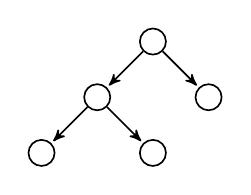
\begin{tikzpicture}[->,>=stealth',shorten >=1pt,auto,node distance=1cm,
                    semithick,initial text=]

  \node[circle,draw]   (0)                    {};
  \node[circle,draw]   (1) [below left of=0]  {};
  \node[circle,draw]   (2) [below right of=0] {};
  \node[circle,draw]   (3) [below left of=1] {};
  \node[circle,draw]   (4) [below right of=1] {};
  
  \path (0) edge              node {} (1)
        (0) edge              node {} (2)
        (1) edge              node {} (3)
        (1) edge              node {} (4);
\end{tikzpicture} \hspace*{2em} Binary Tree!\\[1em]

One characteristic of a binary tree:
\begin{itemize}
\item left \& right pointers don't refer to same node.
\end{itemize}

We can express that characteristic in Java as follows:
\begin{lstlisting}[language=Java]
boolean repOk() {
  if (root == null) return size == 0; 	   	      // empty tree has size 0
  Set visited = new HashSet(); visited.add(root);
  List workList = new LinkedList(); workList.add(root);
  while (!workList.isEmpty()) {
    Node current = (Node)workList.removeFirst();
    if (current.left != null) {
      if (!visited.add(current.left)) return false; // acyclicity
      workList.add(current.left);
    }
    if (current.right != null) {
      if (!visited.add(current.right)) return false; // acyclicity
      workList.add(current.right);
    }
  }
  if (visited.size() != size) return false; 	     // consistency of size
  return true;
}
\end{lstlisting}

Korat then generates all distinct (``non-isomorphic'') trees, 
    up to a given size (say 3).
It uses these trees as inputs for testing 
    the {\tt add()} method of the tree (or for any other methods.)

    \begin{center}
    \url{korat.sourceforge.net/index.html}
  \end{center}



\end{document}
